\documentclass[11pt]{article}

\usepackage{amssymb,amsmath,amsthm}
\usepackage{verbatim}
\usepackage{fullpage}
\usepackage{gencor}
\usepackage{mathrsfs}
\usepackage{authblk}
\usepackage{graphicx}
\usepackage{caption}
\usepackage{subcaption}
\numberwithin{equation}{section}
\usepackage[nottoc,notlof,notlot,numbib]{tocbibind}
\usepackage{xr-hyper}
\externaldocument[supp-]{supp}
\makeatletter
\renewcommand*{\@fnsymbol}[1]{\ensuremath{\ifcase#1\or *\or**\or\dagger\or \ddagger\or
   \mathsection\or \mathparagraph\or \|\or **\or \dagger\dagger
   \or \ddagger\ddagger \else\@ctrerr\fi}}
\makeatother

\frenchspacing
\title{Estimating Genetic Correlation from GWAS Summary Statistics}
\author[1,2,3]{Brendan Bulik-Sullivan\thanks{Co-first authors}$^{\dagger}$}
\author[4,*]{Hilary K Finucane}
\author[1,2,3]{Verneri Antilla}
\author[5,6]{Alexander Gusev}
\author[7]{Felix R. Day}
\author[ ]{the ReproGen Consortium\hspace{-0.7ex}}
\author[7]{John R.B. Perry}
\author[1,2,3]{Cecilia Lindgren}
\author[1]{Nick Patterson}
\author[1,2,3]{Elise Robinson}
\author[1,2,3]{Mark J Daly}
\author[5,6]{Alkes L Price\thanks{Co-last authors}}
\author[1,2,3,**]{Benjamin M Neale\thanks{Correspondence should be addressed to BBS (bulik@broadinstitute.org) or BMN (bmneale@broadinstitute.org).}}

\affil[1]{\small{Program in Medical and Population Genetics, Broad Institute of MIT and Harvard, Cambridge, MA, USA}}
\affil[2]{Stanley Center for Psychiatric Genetics, Broad Institute of MIT and Harvard, Cambridge, MA, USA}
\affil[3]{Analytic and Translational Genetics Unit, Massachusetts General Hospital, Boston, MA, USA.}
\affil[4]{Department of Mathematics, Massachusetts Institute of Technology, Cambridge, MA, USA.}
\affil[5]{Department of Epidemiology, Harvard School of Public Health, Boston, MA, USA.}
\affil[6]{Department of Biostatistics, Harvard School of Public Health, Boston, MA, USA.}
\affil[7]{MRC Epidemiology Unit, University of Cambridge School of Clinical Medicine, Cambridge, UK}
\date{}
\begin{document}
\maketitle



\begin{abstract}

A recent focus in statistical genetics has been leveraging genetic association results from multiple phenotypes simultaneously to assist in the interpretation of results from genome-wide association studies (GWAS). 
Here we describe a novel method for estimating genetic correlations between traits that requires only GWAS summary statistics as input.
We apply our method to 25 sets of publicly available GWAS summary statistics, which include more than 1.5 million phenotyped samples. 
Our results replicate many known genetic and epidemiological associations, including correlations between psychiatric traits, anthropometric traits, and components of metabolic syndrome. 
In addition, we report several novel results, including a positive genetic correlation between anorexia and schizophrenia and a negative genetic correlation between anorexia nervosa (AN) and body mass. 
These results highlight the power of a polygenic modeling framework, since there currently are no genome-wide significant SNPs for AN. 
We provide open source software implementing these analyses.

\end{abstract}
\newpage
%%%%%%%%%%%%%%%%%%%%%%%%%%%%%%%%%%%%%%%%%%%%%%%%%%%%%%%%%%%%%%%
\section{Introduction}
\label{Introduction}
%%%%%%%%%%%%%%%%%%%%%%%%%%%%%%%%%%%%%%%%%%%%%%%%%%%%%%%%%%%%%%%

Discovering relationships between phenotypes is a fundamental goal of epidemiology, with applications to drug development, classification and treatment of disease. 
The traditional strategy in epidemiology is to search for correlations between phenotypes via large cross-sectional or longitudinal observational studies; 
however, the interpretation of results from these studies can be confounded by social factors and reverse causation. 
An alternative strategy that is more robust to confounding is to search instead for pairs of phenotypes with shared genetic etiology \cite{smith2003mendelian}. 
Many such methods have the additional advantage that they do not require measuring the same traits on the same individuals, which is particularly useful for phenotypes that are rare or costly to assay.  
	
The largest currently available sources of genotype-phenotype data are genome-wide association studies (GWAS). 
There are three main approaches for testing relationships between phenotypes using GWAS data. 
Mendelian randomization has proved effective for traits for which there exist large-effect genetic variants \cite{smith2014mendelian}. 
However for many complex traits, the heritability is distributed over thousands of variants with small effect sizes \cite{visscher2012five}. 
For these traits, Mendelian randomization suffers from low power and weak instrument bias \cite{angrist2008mostly}, 
so it is more effective to estimate genetic correlations using techniques such as restricted maximum likelihood (REML) \cite{yang2010, yang2011gcta, lee2012estimation}
or polygenic scores \cite{purcell2009common, dudbridge2013power} that model the effects of all SNPs, including those that do not reach genome-wide significance \cite{pgccdg2013, vattikuti2012heritability, chen2014estimation}.

REML and polygenic scores have only been applied to a small number of traits so far, because these methods requires access to individual genotypes, 
which are often difficult to obtain due to privacy considerations and informed consent limitations. 
Here we introduce a method for estimating genetic correlation that requires only GWAS summary statistics as input and is several orders of magnitude less computationally demanding than REML.

We apply this method to all GWAS for which the summary statistics have been made publicly available for download and report genetic correlations between hundreds of pairs of traits. 
The vast majority of our results are consistent with previously published genetic correlations, observations of overlap at genome-wide significant loci, and epidemiological associations. 
In addition, we report several novel results, including a positive genetic correlation between anorexia and schizophrenia and a negative genetic correlation between anorexia and BMI. 
These results demonstrate the advantages of a polygenic modeling framework, since there are currently no SNPs associated with anorexia at genome-wide significance \cite{boraska2014genome}. 

%%%%%%%%%%%%%%%%%%%%%%%%%%%%%%%%%%%%%%%%%%%%%%%%%%%%%%%%%%%%%%%
\section{Results}\label{Results}
%%%%%%%%%%%%%%%%%%%%%%%%%%%%%%%%%%%%%%%%%%%%%%%%%%%%%%%%%%%%%%%

\subsection{Overview of Methods}

The $\chi^2$-statistic at a given SNP incorporates the effects of all SNPs in LD with that SNP. 
For a polygenic trait, SNPs in regions with strong LD will have higher $\chi^2$ statistics on average than SNPs in regions with little LD \cite{buliksullivan2014}. 
A similar relationship holds if we replace $\chi^2$ statistics for a single trait with the product $z_1z_2$, 
where $z_i$ denotes the $Z$-score for trait $i$.

More precisely, under a polygenic model \cite{yang2010}, the expected value of $z_1z_2$ is 
\begin{equation}\label{reg_eqn}
	\E[z_{1j}z_{2j}] = \dfrac{\sqrt{N_1N_2}\rho_g}{M}\ell_j + \dfrac{\rho N_s}{\sqrt{N_1N_2}},
\end{equation}
where $N_i$ is the sample size for study $i$, $\rho_g$ is genetic covariance, $\ell_j$ is LD Score, $N_s$ is the number of samples shared between study 1 and study 2, and $\rho$ is the phenotypic correlation among the $N_s$ overlapping samples.
A similar relationship holds if one or both of the studies is an ascertained study of a binary phenotype (Supplementary Note), and in this case, the estimate of genetic covariance will be on the observed scale.
As a consequence of equation \ref{reg_eqn}, we can estimate genetic covariance using the slope from the regression of $z_{1j}z_{2j}$ on LD Score. This estimate will not be biased even if the two studies share samples, because sample overlap only 
affects the intercept, not the slope.	
Intuitively, bias from sample overlap affects all SNPs equally, similar to cryptic relatedness in the one-trait case \cite{buliksullivan2014}, and therefore this bias is not correlated with LD Score.

If we normalize genetic covariance to lie in the interval $[-1,1]$, we obtain genetic correlation: 
$r_g := \rho_g/\sqrt{h^2_1h^2_2},$ where $h^2_i$ denotes the heritability of trait $i$. 
In this paper, we report genetic correlations obtained using genetic covariances estimated with two-phenotype LD Score regression
and heritabilities estimated using univariate LD Score regression \cite{buliksullivan2014}.




\subsection{Simulations}\label{Simulations}

We performed a series of simulations to evaluate the robustness of the model to potential confounders such as sample overlap
and misspecified models of genetic architecture, as well as to determine whether the inference procedure produces appropriate type I error, 

\subsection{Misspecified Models of Genetic Architecture}\label{Misspecified Sims}

Estimates of heritability and genetic covariance can be biased if the underlying model of genetic architecture is misspecified
\cite{speed2012improved} 
Estimates of genetic correlation are more robust to model misspecification biases than estimates of 
heritability or genetic covariance. 
Since genetic correlation is estimated as a ratio,
model misspecification biases that affect the numerator and the denominator in the same direction will tend to cancel. 
In situations where MAF- or LD-dependent genetic architectures are a particular concern, it is possible to correct for such biases 
with LD Score regression using a MAF or LD binning approach (see \cite{finucane2014partitioning} and Online Methods)
similar to that taken by Lee, \emph{et. al.} with REML \cite{lee2013estimation}. 

To quantify the bias introduced by MAF- or LD-dependent genetic architectures, we simulated a variety of different LD Scores and genetic architectures.
In realistic scenarios, only a subset of causal SNPs are directly genotyped or successfully imputed, 
so we used a densely imputed panel of 1000 Genomes (1kG) SNPs \cite{10002012integrated} in order to generate phenotypes
and estimate LD Scores, 
but computed summary statistics only for the 16\% of 1kG SNPs that are also in HapMap3 (HM3) \cite{international2010integrating} with MAF above 5\%.
Results from these simulations are displayed in Supplementary Tables 
\ref{supp-parallel}, \ref{supp-antiparallel} and \ref{supp-depcor}.

We found that the partitioned LD Scores were not biased by MAF- and LD-dependent genetic architectures
when estimating heritability and genetic covariance, but gave substantially higher standard errors than non-partitioned LD Scores.
The estimates of genetic correlation from the simpler non-partitioned LD Scores were approximately unbiased in simulations 
where both heritability and genetic covariance depended on LD, and only minimally biased in simulations where genetic 
correlation also depended on LD. In addition, the non-partitioned LD Scores gave substantially lower standard errors than the
more complex partitioned LD Score models.
Thus for the remainder of this paper, we use non-partitioned LD Scores for estimating $r_g$, since these LD Scores had minimal
bias and the lowest variance in simulations.

In all of the simulations described in this section, 
there was full sample overlap, which confirms that the LD Score regression with free intercept is not biased by sample overlap.

\subsection{Replication of PGC Cross Disorder Results}\label{PGCCDG}

For further validation, we replicated the estimates of genetic correlations between psychiatric disorders obtained with
individual genotypes and REML in the Psychiatric Genomics Consortium (PGC) Cross-Disorder Group paper \cite{pgccdg2013}, 
using LD Score regression and the summary statistics from \cite{cross2013identification},
downloaded from the PGC website (URLs).

Including an intercept in the LD Score regression protects the results from QC issues such as population stratification (as described in \cite{buliksullivan2014})
and sample overlap, but at the cost of larger standard errors.
Since the summary statistics from \cite{cross2013identification} were generated after a careful QC process, and the 
samples used for each disease were non-overlapping, we also fit LD Score regression with constrained intercept.

Results from this analysis are displayed in Figure \ref{Fig:Replication of PGC Cross-Disorder Results}.
As expected, the genetic correlation estimates from LD Score regression were similar to the results from REML.
LD Score regression without intercept gave standard errors that were only slightly larger than REML,
while the standard errors from LD Score regression with intercept were larger, especially for smaller sample sizes
(\emph{e.g.,} ADD, ASD).

The computational demands of this analysis were trivial: after computing LD Scores 
(which takes an hour parallelized over chromosomes and only needs to be done once), 
the LD Score regression took a few seconds per pair of phenotypes and less than 1GB of RAM. 

\begin{figure}[!ht]

\begin{centering}
    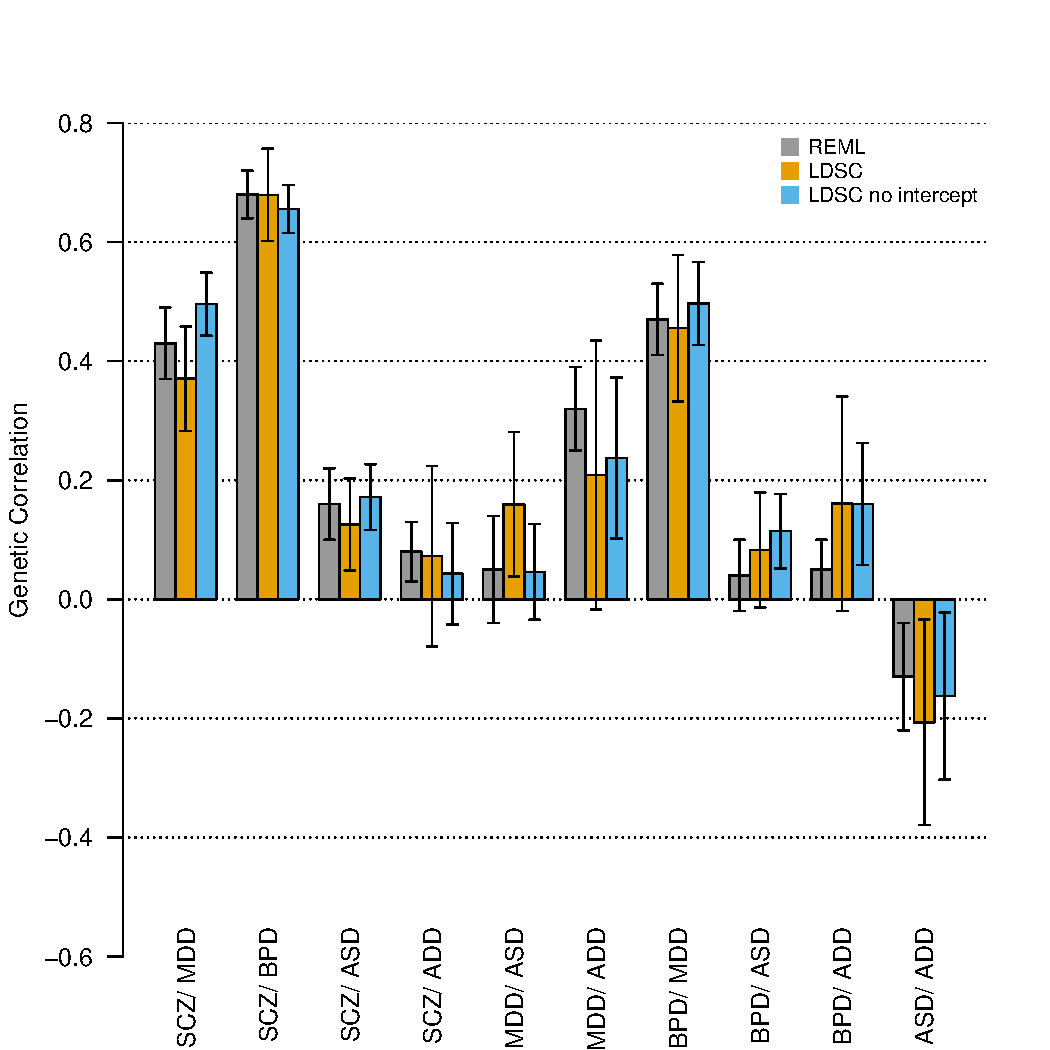
\includegraphics[scale=0.8]{figs/ldsc_vs_gcta.pdf}

\end{centering}

\caption{\label{Fig:Replication of PGC Cross-Disorder Results}\small{\textit{Replication of PGC Cross Disorder Results.
This plot compares LD Score regression estimates of genetic correlation using the summary statistics from \cite{cross2013identification} (which were generated from approximately the same data as \cite{pgccdg2013}) to 
estimates obtained from REML in \cite{pgccdg2013}.
The horizontal axis indicates pairs of phenotypes, and the vertical axis indicates genetic correlation.
The error bars show standard errors.
Colors indicate different estimation procedures. Green is REML,
orange is LD Score with intercept and white is LD Score without intercept.
The estimates of genetic correlation between psychiatric phenotypes in figure \ref{Fig:300 Gencors} use larger sample sizes;
this plot is intended primarily as a technical validation.
Abbreviations: 
ADD = Attention Deficit Hyperactivity Disorder;
ASD = Autism Spectrum Disorder;
BPD = Bipolar Disorder;
MDD = Major Depressive Disorder;
SCZ = Schizophrenia.}}}

\end{figure}

\subsection{Application to a Large Set of Publicly Available Summary Statistics}

We used LD Score regression to estimate genetic correlations between 25 phenotypes (Table \ref{data}, URLs), 
including all phenotypes with publicly available summary statistics and sufficiently large sample size and heritability (see Methods).
For clarity of presentation, we pruned to one phenotype from each cluster of highly correlated phenotypes for the main text; 
highly correlated anthopometric phenotypes are displayed in supplementary table XXX, 
smoking phenotypes are displayed in supplementary table YYY, 
and insulin-related traits are displayed in supplementary table ZZZ. 
Genetic correlation estimates for the 25 traits are displayed in Figure \ref{Fig:300 Gencors}.

\begin{table}[t]

\centering
\begin{tabular}{lllllllll}

Phenotype & Reference & Sample Size \\

  \hline
Schizophrenia  & PGC Schizophrenia Working Group, \textit{Nature,} 2014 \cite{schizophrenia2014biological}  & 70,100\\
Bipolar disorder & PGC Bipolar Working Group, \textit{Nat Genet,} 2011 \cite{sklar2011large} & 16,731\\
Major depression & PGC MDD Working Group, \textit{Mol Psych,} 2013 \cite{ripke2012mega} & 18,759 \\
Anorexia Nervosa & Boraska, \textit{et al.,}  \textit{Mol Psych,} 2014  \cite{boraska2014genome} & 17,767\\
Autism Spectrum Disorder & PGC Cross-Disorder Group, \textit{Lancet,} 2013 \cite{cross2013identification} & 10,263 \\ 
Ever/Never Smoked & TAG Consortium, 2010 \textit{Nat Genet,} \cite{tobacco2010genome}& 74,035 \\
Alzheimer's & Lambert, \textit{et al.,} \textit{Nat Genet,} 2013 \cite{lambert2013meta} & 54,162\\
College & Rietveld, \textit{et al.,} \textit{Science,} 2013 \cite{rietveld2013gwas}& 101,069 \\
Height & Lango Allen, \textit{et al.,}  \textit{Nature} 2010 \cite{allen2010hundreds} &133,858\\
Obesity Class 1 & Berndt, \textit{et al.,} \textit{Nat Genet,} 2013 \cite{berndt2013genome}& 98,000 \\
Extreme Waist-Hip Ratio & Berndt, \textit{et al.,} \textit{Nat Genet,} 2013 \cite{berndt2013genome}& 10,000 \\
Coronary Artery Disease & Schunkert, \textit{et al.,} \textit{Nat Genet,} 2011 \cite{schunkert2011large} & 86,995\\
Triglycerides  & Teslovich, \textit{et al.,} \textit{Nature,} 2010 \cite{teslovich2010biological}& 96,598 \\
LDL Cholesterol & Teslovich, \textit{et al.,} \textit{Nature,} 2010  \cite{teslovich2010biological}& 95,454 \\
HDL Cholesterol& Teslovich, \textit{et al.,}  \textit{Nature,} 2010 \cite{teslovich2010biological}& 99,900 \\
Type-2 Diabetes & Morris, \textit{et al.,}  \textit{Nat Genet,} 2012 \cite{morris2012large} & 69,033  \\
Fasting Glucose & Manning, \textit{et. al.,} \textit{Nat Genet,} 2012 \cite{manning2012genome}& 46,186 \\
Childhood Obesity & EGG Consortium, \textit{Nat Genet,} 2012 \cite{early2012genome}& 13,848 \\
Birth Length & van der Valk, \textit{et al.,} \textit{HMG,} 2014 \cite{van2014novel}& 22,263 \\
Birth Weight & Horikoshi, \textit{et al.,} \textit{Nat Genet,} 2013 \cite{horikoshi2013new}& 26,836 \\ 
Infant Head Circumference & Taal, \textit{et al.,} \textit{Nat Genet,} 2012 \cite{taal2012common}& 10,767 \\
Age at Menarche & Perry, \textit{et al.,} \textit{Nature,} 2014 \cite{perry2014parent}& 132,989\\
Crohn's Disease & Jostins, \textit{et al.,} \textit{Nature,} 2012  \cite{jostins2012host}& 20,883 \\
Ulcerative Colitis & Jostins, \textit{et al.,}  \textit{Nature,} 2012 \cite{jostins2012host}& 27,432 \\
Rheumatoid Arthritis & Stahl, \textit{et al.,} \textit{Nat Genet,} 2010 \cite{stahl2010genome} & 25,708\\
\end{tabular}
\caption{\label{data}
\small{\textit{Datasets used in the main analyses.}}}
\end{table}

\begin{figure}[!ht]

\begin{centering}
    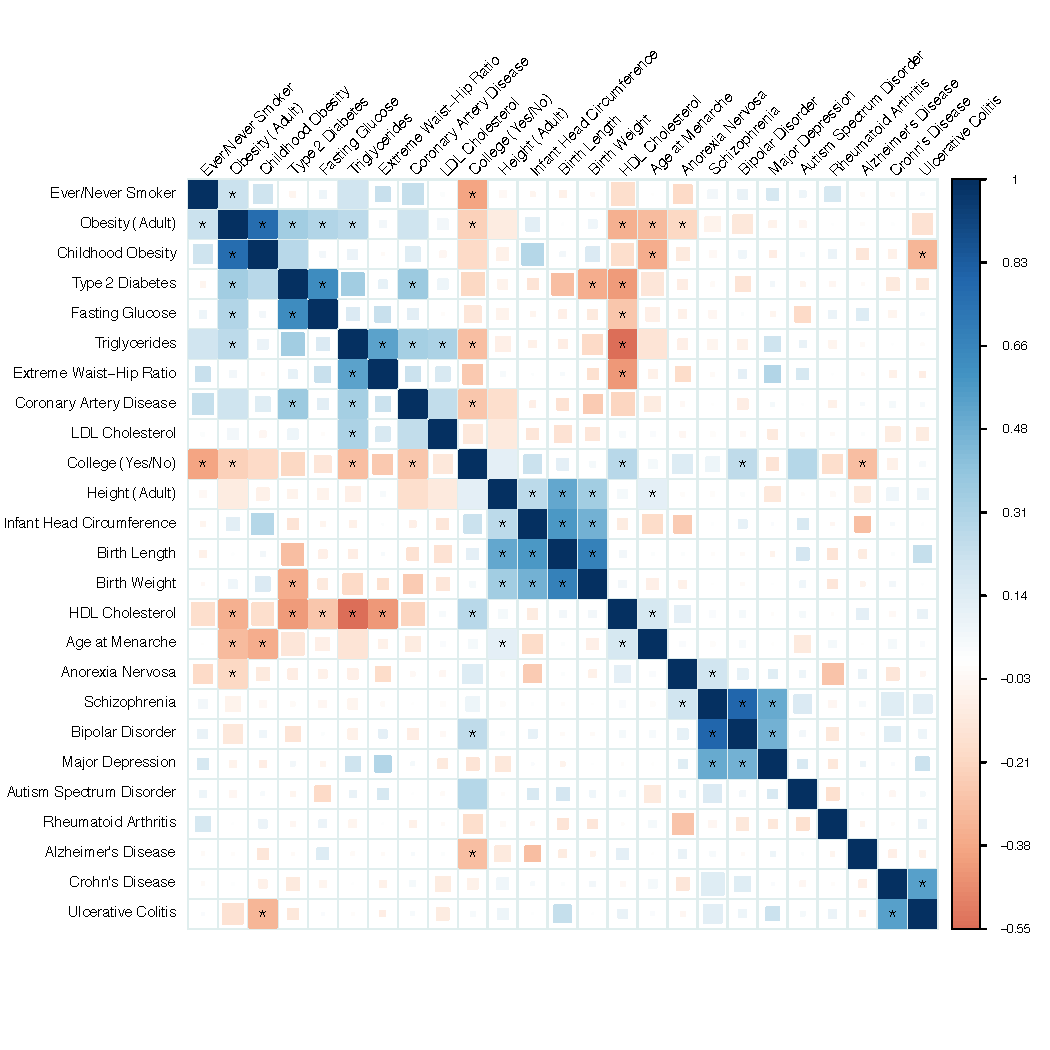
\includegraphics[scale=0.99]{figs/rg_heatmap.pdf}

\caption{         \label{Fig:300 Gencors}
\small{\textit{Genetic Correlations between 25 Published GWAS.
The color of the square indicates the value of the genetic correlation. 
Blue corresponds to positive genetic correlations; red corresponds to negative genetic correlation. 
The size of the colored squares indicates the magnitude of the $p$-value. 
Larger squares correspond to lower $p$-values, and all genetic correlations that are different from zero at 1\% FDR are displayed as full-sized squares. 
Genetic correlations that are significantly different from zero at $\alpha=0.05$ after Bonferroni correction for 300 tests are given an asterisk. 
Note that this multiple testing correction is conservative, since many of the tests are not independent.
}}}

\end{centering}
\end{figure}

% Results that are consistent with previously reported GWAS rg's

Our estimates of genetic correlation between metabolic traits are generally consistent with the estimates obtained using REML in 
\cite{vattikuti2012heritability}, though our standard errors are much lower, since operating on summary statistics
allows us access to larger sample sizes (Supplementary Table \ref{supp-vattikuti}). 
In addition, our estimate of 0.57 (0.074) for the genetic correlation between Crohn's disease and ulcerative colitis is consistent
with the estimate of 0.62 (0.042) from \cite{chen2014estimation}.

% Results that are consistent with top SNP results or MR analyses 

For the majority of pairs of traits in Figure \ref{Fig:300 Gencors}, no GWAS-based genetic correlation estimate has been reported; 
however, many associations have been described in an \emph{ad-hoc} manner based off the observation of overlap among genome-wide significant loci, 
or, more formally, via Mendelian randomization analyses. 
Examples of genetic correlations that are consistent with overlap among top loci include the correlations between plasma lipids and cardiovascular disease \cite{do2013common}; age at onset of menarche and obesity \cite{perry2014parent}; type 2 diabetes and obesity, fasting glucose, plasma lipids, and cardiovascular disease \cite{morris2012large}; birth weight, adult height and type 2 diabetes \cite{horikoshi2013new}; birth length, adult height and infant head circumference \cite{early2012genome, taal2012common}; and childhood obesity and adult obesity \cite{early2012genome}. 
For many of these pairs of traits, we can reject the null hypothesis of zero genetic correlation with overwhelming statistical
significance (\emph{e.g.,} $p=6\times10^{-24}$ for age at onset of menarche and obesity; $p=6\times10^{-52}$ for obesity and childhood obesity).

Our results on metabolic traits are directionally consistent with the recent Mendelian randomization results from \cite{wuertz2014metabolic}, except that we identify a statistically significant positive genetic correlation between fasting glucose and obesity, and they identify a positive effect of BMI on LDL that is not apparent in our data. 
Some of these results have also been reported in the twin study literature; for example, our estimate of 0.12 (0.03) ($p=5\times10^{-4}$) for the genetic correlation between adult height and educational attainment is consistent with the genetic correlation estimates of 0.08 in males and 0.17 in females between adult height and IQ (for which educational attainment is a proxy phenotype) from \cite{keller2013genetic}. 
This result has also been reported in the epidemiological literature \cite{magnusson2006height}, 
though we stress that this genetic correlation should not be given a causal interpretation.
Both height and educational attainment have genetic correlations with many other phenotypes, 
and the observed genetic correlation between height and educational attainment could be mediated by any of these (see Discussion).
The negative genetic correlation between birth weight and type 2 diabetes that we report is also consistent with overlap among top loci observed in \cite{johansson2008association}.

% Novel genetic results that are not novel epidemiological results

Many of our results are consistent with well-known epidemiological association, but, to the best of our knowledge, have never been reported using genetic data.
For example, our estimates of the genetic correlation between age at onset of menarche and adult height \cite{onland2005age}, cardiovascular disease \cite{day2014} and type 2 diabetes \cite{day2014, elks2013age} are consistent with the epidemiological associations. 
We estimate a genetic correlation of -0.30 (0.08), $p=1\times10^{-4}$, between educational attainment and Alzheimer's disease, 
consistent with the epidemiological observation that low educational attainment is one of the largest risk factors for Alzheimer's
\cite{barnes2011projected, norton2014potential}. 
The positive genetic correlation between educational attainment and bipolar disorder is consistent with psychiatric literature showing that education and bipolar disorder status are positively correlated
\cite{maccabe2010excellent, tiihonen2005premorbid}, 
Our estimate of a genetic correlation of -0.20 (0.04) ($p=4\times10^{-6}$) between anorexia and obesity is sensible considering that low BMI is one of the diagnostic criteria for anorexia, though it is interesting that the genetic factors that influence normal variation in BMI are similar to the genetic factors that influence unhealthily low BMI in the context of psychiatric illness.
This result is consistent with our observation that BMI GWAS findings appear to primarily implicate neuronal, rather than metabolic, cell-types and epigenetic marks 
\cite{finucane2014partitioning}.
Our estimate of the genetic correlations between schizophrenia and inflammatory bowel disease (IBD -- Crohn's and UC) are not statistically significantly different from zero after correction
for multiple tests, but the direction of the genetic correlation (positive) is consistent with recent epidemiological work showing an increased risk for schizophrenia after IBD diagnosis
\cite{benros2011autoimmune} and an increased risk for IBD after schizophrenia diagnosis \cite{benros2014nationwide}.
These observations are particularly interesting in light of recent results showing that immune cell-type-specific epigenetic marks are enriched for genetic variants that influence risk
for schizophrenia \cite{finucane2014partitioning, schizophrenia2014biological}, although we emphasize that the evidence for genetic correlation is not yet conclusive.
The positive genetic correlation between smoking and obesity is in the opposite direction of the epidemiological association (smoking is associated with lower body mass, although smoking cessation 
often leads to weight gain) and Mendelian randomization results using rs1051730 \cite{aasvold2014causal}.
We propose that the resolution of this apparent discrepancy is an interesting direction for future research.
Our estimate of a negative genetic correlation between smoking and educational attainment is consistent with the epidemiological result that smoking is more prevalent among less-educated groups \cite{pierce1989trends}.
Last, the genetic correlation of -0.17 (0.04) ($p=2\times10^{-4}$) between height and coronary artery disease (possibly related to the genetic correlation of -0.11 (0.03) ($p=0.001$) between height and LDL, a known risk factor for coronary artery disease \cite{do2013common, burgess2014using}) is consistent with a replicated epidemiological association  \cite{wang2011associations,hebert1993height,rich1995height}.

% Novel results

We report three results that are, to the best of our knowledge, novel.
First, we found a genetic correlation of 0.19 (0.04) between between anorexia nervosa and schizophrenia ($p=1.5\times10^{-5}$).
Suggestive evidence for comorbidity between anorexia nervosa and schizophrenia has been reported previously \cite{striegel1999psychiatric,blinder2006psychiatric}.
This raises the intriguing possibility of a fundamental similarity between these disorders, despite many differences in clinical course, sex ratios, and response to antipsychotics.
%%% Getting citations from my parents 

Second, we estimate a genetic correlation of -0.33 (0.08) between ulcerative colitis and childhood obesity ($p=3.9\times10^{-5}$). 
We suggest that this should be interpreted with caution, given the unusually high LD Score regression for UC (intercept 1.07  compared to mean $\chi^2$ of 1.19).
This either indicates substantial confounding due to population stratification or (more likely) that the LD Score regression model is a poor fit for the genetic architecture of UC,
which features many low frequency variants with large odds ratios.
Third, we estimate a genetic correlation of 0.28 (0.08) ($p=5\times10^{-4}$) between autism spectrum disorder (ASD) and educational attainment (a proxy for intelligence \cite{rietveld2013gwas}).
The ASD summary statistics were generated using a case/pseudocontrol study design, so this result cannot be explained by diagnostic biases, such as the tendency for the parents of children who receive a diagnosis of ASD to be better educated than the general population \cite{durkin2010socioeconomic}. The distribution of IQ among individuals with ASD has lower mean than the general population, but with heavy tails \cite{robinson2014autism} (\emph{i.e.,} an excess of individuals with extremely low and extremely high IQ).
In addition, there is evidence that the genetic architectures of high IQ and low IQ ASD are dissimilar \cite{samocha2014framework}.
We are unable to offer an explanation for this result, but propose that further exploration of this genetic correlation is an interesting direction for future research.

% Interesting negative results

Finally, we report several instances where the genetic correlation is close to zero, in contrast to previous reports of epidemiological correlation or genetic overlap.
We estimate genetic correlations close to zero between schizophrenia and rheumatoid arthritis, schizophrenia and smoking, and schizophrenia and plasma lipids. The lack of genetic correlation between schizophrenia and rheumatoid arthritis is interesting because schizophrenia has been observed to be protective for rheumatoid arthritis \cite{silman2002epidemiology}.
The absence of genetic correlation between schizophrenia and smoking is notable because of the high prevalence of smoking among individuals with schizophrenia \cite{de2005meta}. 
Our estimate of zero genetic correlation between schizophrenia and plasma lipids or cardiovascular disease contrasts with earlier reports of extensive pleiotropy between schizophrenia and triglycerides \cite{andreassen2013improved2}, which may have been artifacts of inadequate control for LD (see Discussion). 
%%% Waiting to hear back from Sasha about the current state of the comparison to the Andreassen conditional QQ plot method
Last, we estimate near zero genetic correlation between rheumatoid arthritis and both Crohn's disease and ulcerative colitis. Although these immune diseases share a large number of associated loci, it appears that the directions of effect are in the opposite direction as often as they are concordant, yielding close to zero genetic correlation overall.
%%% Getting # of overlapping gwsig loci w/ concordant and discordant effects from Mark 


%%%%%%%%%%%%%%%%%%%%%%%%%%%%%%%%%%%%%%%%%%%%%%%%%%%%%%%%%%%%%%%
\section{Discussion}\label{Discussion}
%%%%%%%%%%%%%%%%%%%%%%%%%%%%%%%%%%%%%%%%%%%%%%%%%%%%%%%%%%%%%%%\


% Summary of major findings
We have described a new method for estimating genetic correlation from GWAS summary statistics.
This method is an advance for five  main reasons: it does not require individual genotypes; it does not require genome-wide significant SNPs; it is not biased by sample overlap; it does not require measuring all phenotypes on all individuals, and it is is computationally trivial.  
These advantages allow estimation of genetic correlations between a much large set of pairs of phenotypes than was previously possible.

% Importance of findings 
We applied our method to a large dataset of publicly available GWAS summary statistics, spanning 25 traits and more than 1.5 million phenotyped individuals. 
We replicated many previously-reported GWAS-based genetic correlations, observations of overlap among genome-wide significant SNPs, and known epidemiological associations, thus validating the utility of genetic correlation as an epidemiological tool.
In addition, we report several novel results, including a positive genetic correlation between educational attainment and ASD, 
which may be related to emerging differences between the genetic architectures of high IQ and low IQ ASD. 

% Limitations of Genetic Correlation
We note some limitations on the interpretation of genetic correlation.
In general, the difficulties in interpreting genetic correlation are similar to the difficulties in interpretation of Mendelian randomization.
Although genetic correlation is immune to environmental confounding, genetic correlation is still subject to genetic confounding. 
This is best illustrated with an example. 
Consider the strong negative genetic correlation between HDL and CAD in Figure \ref{Fig:300 Gencors}.
This genetic correlation could result from a direct causal effect $\mathrm{HDL}\rightarrow\mathrm{CAD}$,
but could also result from non-causal shared genetic etiology, perhaps mediated by the strong genetic correlation of -0.55 between HDL and triglycerides (TG). 
This scenario can be represented graphically as 
$\mathrm{HDL}\leftarrow\mathrm{G}\rightarrow\mathrm{TG}\rightarrow\mathrm{CAD}$, 
where $\mathrm{G}$ is the set of genetic variants with effects on both HDL and TG.
Indeed, the second mechanism appears to account for a large proportion of the genetic correlation between HDL and CAD, 
since the association between HDL and CAD is attenuated after controlling for other plasma lipids \cite{do2013common, burgess2014using}.
Extending genetic correlation to deal with multiple phenotypes (\emph{e.g.,} genetic correlation between HDL and CAD controlling for TG, 
analogous to \cite{do2013common,burgess2014using}, possibly with extension to nonlinear models) is an important direction for future work.

% Limitations of the Method

We note several limitations of the LD Score regression method.
First, LD Score regression requires large sample sizes in order to give estimates with reasonable standard error 
(as a rule of thumb, $Nh^2_g$ should be greater than 3000, where $h^2_g$ is on the observed scale for case/control studies).
Constrained intercept LD Score regression gives lower standard errors, 
but this estimator requires knowing the number of overlapping samples, which can often be difficult to determine for pairs of large meta-analyses.
REML and genetic risk scores are more efficient estimators of genetic correlation, though both require access to individual genotypes.
Second, LD Score regression assumes that all individuals in the GWAS were sampled from populations with similar LD Scores,
and that these LD Scores can be estimated from sequenced reference data such as 1kG.
Differences between LD patterns in the reference panel and the GWAS sample may result in bias \cite{buliksullivan2014}. 
Third, there is currently no procedure for applying LD Score regression to samples from admixed populations.
Fourth, LD Score regression performs optimally when applied to traits with highly polygenic genetic architectures, such as 
psychiatric traits. 
At large sample size and for less-polygenic traits (\emph{e.g.,} traits where a substantial fraction of heritability is concentrated among a handful of SNPs), 
it is sometimes possible to obtain better power by analyzing only the large-effect SNPs. 
Developing methods that can make optimal use of both confidently associated large-effect SNPs and diffuse polygenic signal from thousands of small-effect SNPs is a direction for future research.
Fifth, while LD Score regression is a consistent estimator of genetic correlation in ascertained case/control studies,
the results may nonetheless be skewed by more subtle biases in ascertainment, such as misclassification of cases.

Finally, we have developed a method that allows us to rapidly screen hundreds of pairs of phenotypes for associations without having to measure all phenotypes on all individuals.
Our results show that the matrix of genetic correlations -- especially among metabolic traits -- is dense, and that 
genome-wide genetic pleiotropy is the rule rather than the exception.
These findings highlight the importance of methods that account naturally for pleiotropy \cite{do2013common, burgess2014using},
or even use pleiotropy to gain power \cite{zhou2014efficient, cotsapas2011pervasive}.

\newpage
%%%%%%%%%%%%%%%%%%%%%%%%%%%%%%%%%%%%%%%%%%%%%%%%%%%%%%%%%%%%%%%
\section{Online Methods}\label{Online Methods}
%%%%%%%%%%%%%%%%%%%%%%%%%%%%%%%%%%%%%%%%%%%%%%%%%%%%%%%%%%%%%%%

%%%%%%%%%%%%%%%%%%%%%%%%%%%%%%%%%%%%%%%%%%%%%%%%%%%%%%%%%%%%%%%
\subsection{Statistical Framework}
%%%%%%%%%%%%%%%%%%%%%%%%%%%%%%%%%%%%%%%%%%%%%%%%%%%%%%%%%%%%%%%

A discussion of modeling assumptions and a derivation of the two-phenotype LD Score regression equation 
is provided in the Supplementary Note. 
This section focuses on definitions of quantitates estimated and details of the estimation procedure.

\subsection{Heritability}

Let $S$ denote a set of $M$ SNPs, 
let $X$ denote the random $M$-vector of additively (0-1-2) coded genotypes for the SNPs in $S$, 
and let $y$ denote a phenotype. Define 
\begin{equation}
	\beta := \mathrm{argmax}_{\alpha\in\R^M} \corr\left[y, X\alpha\right]^2,
\end{equation}
where the maximization is performed in the population (\emph{i.e.,} at infinite sample size), rather than in a finite sample.
This is a projection, so uniqueness of $\beta$ is guaranteed as we remove SNPs that are linearly dependent (in the population). 
Then $h^2_S$, the heritability accounted for by SNPs in $S$, is defined
\begin{equation}\label{h2}
	h^2_S := \sum_{j=1}^M \beta_j^2.
\end{equation}
We obtain the Yang/Visscher parameter $h^2_g$ by taking $S$ to be the set of genotyped SNPs.
If we let $S$ denote the set of all SNPs in 1000 Genomes Europeans \cite{10002012integrated}, 
and let $S'$ denote the set of SNPs with MAF$>5\%$, then
\begin{equation}
	h^2_{5\myhyphen50\%} := \sum_{j\in S'} \beta_j^2.
\end{equation}
We choose 5\% as the lower bound, because we can estimate LD Scores for 5\% SNPs reasonably well from the $N=387$ 
samples in 1000 Genomes. 
Technically, we should write $h^2_{5\myhyphen50\%,1kG}$ to indicate that we are only accounting for SNPs in 1000 Genomes,
but 1000 Genomes has sufficiently good power to observe 5\% and higher SNPs that we feel justified in omitting 1kG from the subscript.
With larger sample sizes in future sequenced reference panels, this lower bound can be pushed lower.

There are two main distinctions between $h^2_{5\myhyphen50\%}$ and $h^2_g$,
First, $h^2_g$ does not include the effects of common SNPs that are not tagged by the set of genotyped SNPs $g$.
Second, the effects of causal 4\% SNPs are not counted towards $h^2_{5\myhyphen50\%}$.
In practice, neither of these distinctions makes a large difference, since most GWAS arrays focus on common variation
and manage to assay or tag almost all common variants.

Estimating $h^2_{5\myhyphen50\%}$ involves only as simple modification of LD Score regression: the raw slope from the 
regression divided by sample size yields an estimate of the average value of $\beta^2_j$. 
If we multiply this number by $M$, the number of SNPs in 1000 Genomes, then technically we obtain an estimate of the 
heritability explained by all 1000 Genomes SNPs; however, this interpretation amounts to assuming that 
our estimate of heritability per SNP obtained from common SNP GWAS data also applies to rare variants.
This is unreasonable, since GWAS data contains very little information about rare variants, 
Therefore, we instead multiply the slope by $M_{5\myhyphen50\%}$, the number of 1000 Genomes SNPs with 
MAF between 5\% and 50\%, in order to obtain an estimate of $h^2_{5\myhyphen50\%}$.
The default option in \texttt{ldsc} is to estimate $h^2_{5\myhyphen50\%}$; this can be overridden with the 
\texttt{--not-M-5-50} flag.

The value of $h^2_{5\myhyphen50\%}$ will always be less than the total narrow-sense heritability, $h^2$, 
since $h^2$ takes into account all forms of genetic variation 
-- variants with MAF under 5\%, microsatellites, indels, copy number variants -- not just common SNPs.
In addition, estimates of $h^2$ from family studies may 
be biased upwards by non-additive genetic architectures \cite{zuk2012mystery}.
 
\subsection{Genetic Covariance and Correlation}

For this section, we keep the same notation from the previous section, except with two phenotypes
$y_1$ and $y_2$.
Define
\begin{equation}\label{beta}
	\beta := \mathrm{argmax}_{\alpha\in\R^M}\corr[y_1, X\alpha]^2,
\end{equation}
and 
\begin{equation}\label{beta2}
	\gamma := \mathrm{argmax}_{\alpha\in\R^M}\corr[y_2, X\alpha]^2,
\end{equation}
Then the genetic covariance among SNPs in $S$ is defined
\begin{equation}
	\rho_S := \sum_{j\in S} \beta_j\gamma_j,
\end{equation}
Next, let $S$ denote the set of all SNPs in 1000 Genomes Europeans \cite{10002012integrated}, 
and let $S'$ denote the set of SNPs with MAF$>5\%$. Then
\begin{equation}
	\pf := \sum_{j\in S'} \beta_j\gamma_j.
\end{equation}

The distinctions between these quantities are the same as the distinctions between $h^2_g$ and $\hf$.
Rescaling genetic covariance to lie in the range $[-1,1]$ makes it easier to interpret, so it is more common to instead report 
genetic correlation,
\begin{equation}\label{EQN: rg}
	r_S := \dfrac{\rho_S}{\sqrt{h^2_{S,1}h^2_{S,2}}}.
\end{equation}
The quantity $\rf$ is defined by replacing $S$ with $5\myhyphen50\%$ in equation \ref{EQN: rg}.
As a practical matter, the difference between $r_g$ (the genetic correlation among genotyped SNPs)
and $\rf$ will be quite small when $g$ contains a large proportion of all common SNPs.
This is supported by the simulations described in Section \ref{Misspecified Sims} of the main text. 
Technically, LD Score regression with HM3 LD Score is an estimator of $r_{HM3(5\myhyphen50\%)}$,
the genetic correlation among SNPs in HM3 with MAF between 5 and 50\%, but the resulting estimates
of genetic correlation were almost identical to the estimates of $r_{1kG(5\myhyphen50\%)}$ obtained with 1kG LD Scores
(Supplementary Tables \ref{supp-parallel}, \ref{supp-antiparallel} and \ref{supp-depcor}), 
which is why we do not emphasize this distinction in the main text.

It is however important to note that all of the flavors of GWAS genetic covariance and correlation 
($\rho_g$, $\pf$, $r_g$ and $\rf$) are different from the quantities estimated from family studies.
In a family study, the relationship matrix captures information about all genetic variation, not just common SNPs,
so family studies attempt to estimate the total narrow-sense genetic covariance and the total narrow-sense
genetic correlation. 
Unlike the relationship between $h^2_g$ or $\hf$ and the total narrow-sense heritability $h^2$, there is no simple inequality
relating $r_g$ and $\rf$ to the total narrow-sense genetic correlation.
For example, if $\beta$ and $\gamma$ are strongly correlated among common variants, but only weakly correlated among rare
variants, then the total narrow-sense genetic correlation will be less than $r_g$ and $\rf$.

\subsection{Genetic Correlation is Different from Pleiotropy}

Genetic correlation is defined as the correlation across SNPs of additive per-normalized genotype effect sizes for two traits.
Pleiotropy is defined as the tendency for the same variants to have nonzero effects on two or more phenotypes. 
Genetic correlation is a strictly stronger condition than pleiotropy:
to exhibit genetic correlation, it is not sufficient for two phenotypes to be influenced by the same genetic variants,
the directions of effects must also be consistently aligned across the genome.

Nevertheless, both quantities are informative. 
If two phenotypes are influenced by variants at the same loci or in the same pathways, this may well indicate interesting
shared biology, even if the direction of the effects do not align. 
However, quantifying genome-wide pleiotropy from GWAS summary statistics remains an open challenge
\cite{solovieff2013pleiotropy}. 
For example, since $p$-values tend to decrease with LD Score \cite{buliksullivan2014} and near coding and regulatory
regions \cite{gusevregulatory}, the observation that low $p$-values for one phenotype tend to predict low $p$-values for another 
(as in \cite{schork2013all, andreassen2013improved, andreassen2013improved2})
may merely reflect properties shared by almost all pairs of heritable phenotypes, 
rather than a special property of a specific pair of phenotypes 
(Supplementary Figures \ref{supp-pleiotropy}, \ref{supp-qq_tg}, \ref{supp-qq_bip}).
Genetic correlation estimates from LD Score regression are not affected by these concerns, and so may be more 
easily interpretable than currently-available estimates of genome-wide pleiotropy.

\subsection{Two-Phenotype LD Score Regression}
The method described in this paper is based on a simple regression equation relating the product of $Z$-scores of a given SNP from two GWAS's to the LD Score of the SNP, the genetic correlation and the phenotypic correlation. 
Precisely, let $z_{1,j}$ and $z_{2,j}$ be the $Z$-scores for a SNP $j$ from two GWAS's, and let $\ell_j$ be the LD Score of SNP $j$; 
\emph{i.e.,} $\ell_j = \sum_k r^2(j,k)$.
Then, assuming a simple model of genetic architecture where for each phenotype, SNP effect sizes are drawn in an uncorrelated fashion from distributions with mean zero and a fixed variance and covariance, we have
\begin{equation}
\label{eq.main}
		\E[z_{1,j}z_{2,j}] = \dfrac{\rho_g\sqrt{N_1N_2}}{M}\ell_j + \dfrac{\rho N_s}{\sqrt{N_1N_2}},
\end{equation}
where $N_1$ and $N_2$ are the sample sizes of the two studies, $N_s$ is the number of shared samples,
$\rho$ is the overall phenotypic correlation and $\rho_g$ is the genetic covariance. Since sample overlap affects the term $z_{1,j}z_{2,j}$ equally for all SNPs, and the quantity $N_s$ appears only in the intercept term.
Equation~\eqref{eq.main} is derived in the Supplementary Note. 

We can therefore estimate the genetic covariance, $\rho_g$, by regressing $z_{1,j}z_{2,j}$ against $\ell_j$, 
and multiplying the resulting slope by $M/\sqrt{N_1N_2}$. 
Because sample overlap only affects the intercept of this regression, 
and the LD Score regression estimator of genetic covariance is based on the slope,
the LD Score regression estimator of genetic covariance is not biased by sample overlap. 
Indeed, if $\rho$ is known (\emph{e.g.,} if both studies assay the same phenotype and $\rho=1$), the intercept 
from this regression times a constant can be used as an estimator of the number of shared samples.
Alternatively, if both $N_s$ and $\rho$ are known ahead of time, constraining the intercept can substantially reduce the 
standard error, though this also has the side effect of removing the robustness to shared population stratification.
Constraining the intercept is accomplished via the \texttt{--no-intercept} or \texttt{--constrain-intercept} flags in \texttt{ldsc}.

We can estimate heritability using LD Score regression (as described in \cite{buliksullivan2014}),
and use these heritability estimates to transform the estimates of genetic covariance into estimates of genetic correlation
(see Section \ref{Block Jackknife} in the Methods).

An equation similar to Equation~\eqref{eq.main} holds if one or both of the studies 
is an ascertained study of a binary phenotype, and so the same method can be used regardless of whether the $Z$-scores are from studies of quantitative or case-control traits (Supplementary Note). 
If the variance of effect sizes depends on minor allele frequency (MAF) or linkage disequilibrium (LD), as discussed in \cite{speed2012improved, buliksullivan2014}, this can introduce model misspecification bias into estimates of heritability
and genetic correlation from methods such as LD Score regression and REML. 
However, we can easily accommodate MAF- and LD-dependent genetic architectures using partitioned LD Score regression,
as described in the results and methods sections as well as \cite{finucane2014partitioning}. 


%%%%%%%%%%%%%%%%%%%%%%%%%%%%%%%%%%%%%%%%%%%%%%%%%%%%%%%%%%%%%%%
\subsection{Genetic Covariance Regression Weights} 
%%%%%%%%%%%%%%%%%%%%%%%%%%%%%%%%%%%%%%%%%%%%%%%%%%%%%%%%%%%%%%%

For heritability estimation, we use the LD Score regression weights derived in the 
Supplementary Note from \cite{buliksullivan2014}. 
If effect sizes for both phenotypes are drawn from a bivariate normal distribution, then
the optimal regression weights for genetic covariance estimation are 
\begin{equation}
\var[\bhat_j\chat_j \,|\, \ell_j ] = 
	\left( 
		\frac{\hsqo\ell_j}{M} 
		+ 
		\frac{1}{N_1} 
	\right) \left(  
		\frac{\hsqt\ell_j}{M} 
		+ 
		\frac{1}{N_2}
	\right) 
	+ 					
	2\left( 
		\frac{\gencov\ell_j}{M} 
		+ 
		\frac{\rho N_s}{N_1N_2} 
	\right)^2;
\end{equation}
(Supplementary Note) however, this quantity depends on both heritabilities, 
the genetic covariance and the number of overlapping samples,
which are not known a priori, so it is necessary to estimate them from the data.
Linear regression with weights estimated from the data is feasible generalized least squares (FGLS),
which gives valid inference. 

In order to estimate genetic covariance with efficient regression weights, we run a first LD Score 
regression weighted with weights computed using the heritability estimates from the single-phenotype LD Score regressions,
$N_s$ set to zero, and $\rho_g$ estimated with the aggregate estimator 
$$\hat{\rho}_{g, agg} := \frac{1}{\lbar\sqrt{N_1N_2}}\sum_{j=1}^M z_{1,j}z_{2,j},$$
where $\lbar$ denotes the mean LD Score among SNPs included in the regression.

We then update the weights using the estimates of $\rho_g$ and $\rho N_s$ obtained from the first LD Score regression.

%%%%%%%%%%%%%%%%%%%%%%%%%%%%%%%%%%%%%%%%%%%%%%%%%%%%%%%%%%%%%%%
\subsection{Weighted Block Jackknife Genetic Correlation}\label{Block Jackknife}
%%%%%%%%%%%%%%%%%%%%%%%%%%%%%%%%%%%%%%%%%%%%%%%%%%%%%%%%%%%%%%%

This section describes the implementation of the \texttt{--rg} flag in \texttt{ldsc}.
Genetic correlation is defined as a ratio of quantities: 
\begin{equation*}
	r_g := \frac{\gencov}{\sqrt{\hsqo\hsqt}}.
\end{equation*}
Instead of the naive estimator of this ratio, 
\begin{equation*}
	\rhat_{g} := \frac{\hat{\rho}_g }{ \sqrt{\hat{h}^2_1\hat{h}^2_2}},
\end{equation*}
we use the weighted block jackknife estimator \cite{busing1999delete} of the ratio, 
with the jackknife taken over blocks of adjacent SNPs
\begin{equation}
    \hat{r}_{g,jack} := 
    n_b\hat{r}_{g} -
     \sum_{i=1}^{n_b}
     	\left(1-\frac{m_i}{M_g}\right)\hat{r}_{g,i}
\end{equation}
where $n_b$ is the number of blocks, and $\hat{r}_{g,i}$ is
the naive estimate of genetic correlation obtained by deleting the $i^{th}$ block of SNPs, 
$m_i$ is the number of SNPs in block $i$, and $M_g$ is the number of SNPs included in the regression.
The weighted block jackknife ratio estimator is less biased than the naive estimate 
(though this is not so important at the sample sizes that we consider), 
and comes with a convenient nonparametric heteroskedasticity- and correlation-robust variance estimator \cite{busing1999delete},
\begin{equation}
    \widehat{\mathrm{Var}}\left[\hat{r}_{g,jack}\right] 
:= 
    \frac{1}{n_b} \sum_{i=1}^{n_b}
    	\frac{1}{h_i - 1}
	\left(
		(h_i-n_b)\hat{r}_g - (h_i-1)\hat{r}_{g,i} + \sum_{j=1}^{n_b} \left(1-\frac{m_i}{M_g}\hat{r}_{g,j}\right)
		\right),
\end{equation}
where $h_i := M_g / m_i$.
Weighted block jackknife standard errors (over blocks of adjacent SNPs) 
are robust to the  correlated error structure of GWAS $\chi^2$-statistics, 
so long as the block size exceeds the typical range of LD. 
See references \cite{buliksullivan2014, finucane2014partitioning, moorjani2011history} 
for examples of papers in the statistical and population genetics literature that use this technique. 
We checked the reliability of our standard errors via simulations with real genotypes
(Supplementary Table \ref{supp-se_sim}),
and found that the \texttt{ldsc} default setting  of 2000 blocks genome-wide
(which can be adjusted with the \texttt{--num-blocks} flag) gives standard error estimates
that agree well with the empirical standard deviation across simulation replicates,
even though many of the SNPs included in the regression are in LD.

The standard error of the genetic correlation estimate depends not only on sample size but also heritability.
As a rule of thumb, the higher the heritability $Z$-score ($\hat{h}^2/\mathrm{se}(\hat{h}^2)$), the lower the standard error for genetic correlation.
This is a general feature of ratio estimators and is not specific to LD Score regression;
it is always difficult to obtain an accurate estimate of $1/x$ when the random variable $x$ is close to zero.

In another set of simulations with much lower power (not shown), we observed that the LD Score regression
genetic correlation estimates became unstable when either sample size or heritability was so low that at least one 
of the two heritability estimates was not significantly different from zero. 
This is a general difficult with attempting to estimate a ratio where the denominator is close to zero, and is not 
specific to LD Score regression. 
As a rule of thumb,  we recommend discarding any genetic correlation estimates
where of the block jackknife SE for the genetic correlation estimate is greater than 0.25.
If this occurs, \texttt{ldsc} will print an error message by default.

%%%%%%%%%%%%%%%%%%%%%%%%%%%%%%%%%%%%%%%%%%%%%%%%%%%%%%%%%%%%%%%
\subsection{Complexity}
%%%%%%%%%%%%%%%%%%%%%%%%%%%%%%%%%%%%%%%%%%%%%%%%%%%%%%%%%%%%%%%

If $N$ denotes sample size and $M$ denotes the number of SNPs, then LD Score regression takes
$\mathscr{O}(MN)$ time for computing summary statistics and $\mathscr{O}(M)$ time for the regression. 
Estimating LD Scores takes $\mathscr{O}(MN)$ time, though $N$ for estimating LD Scores does not need to as large as $N$
for GWAS; for instance, we use $N=378$ Europeans from 1000 Genomes for estimating LD Score. 
In addition, LD Scores only need to be computed once, and can then be applied to many pairs of phenotypes.

Practically, estimating LD Scores takes about an hour parallelized over chromosomes, and
LD Score regression takes about one minute for each pair of phenotypes on a standard laptop, 
most of which is spent reading files into memory.

For comparison, REML takes time $\mathscr{O}(MN^2)$ for computing the genetic relatedness matrix (GRM)
and $\mathscr{O}(N^3)$ time for maximizing the likelihood.

%%%%%%%%%%%%%%%%%%%%%%%%%%%%%%%%%%%%%%%%%%%%%%%%%%%%%%%%%%%%%%%
\subsection{Selection of Datasets}
%%%%%%%%%%%%%%%%%%%%%%%%%%%%%%%%%%%%%%%%%%%%%%%%%%%%%%%%%%%%%%%

We selected traits for inclusion in the main text via the following procedure:

\begin{enumerate}
\item Begin with all publicly available non-sex-stratified European-only summary statistics that provide signed summary statistics, are imputed to at least HapMap 2 and do not include heritable covariates.
\item Remove all traits with heritability $Z$-score below 4, in order to remove traits where the genetic correlation estimates will be too noisy to interpret.
\item Prune sets of highly correlated phenotypes (\emph{e.g.,} obesity classes 1-3, or the several glucose and insulin measures from the MAGIC consortium) by picking the trait from each cluster with the highest heritability heritability $Z$-score (traits pruned in this step are displayed in the supplementary figures).

\end{enumerate}

\subsection{Summary Statistics}\label{Summary Statistics}

The minimum summary data required for estimating genetic correlation with LD Score regression are the following:
\begin{enumerate}
	\item Genome-wide summary statistics from cohorts with similar ancestry
	\item The summary statistics must be \emph{signed} (allele and direction of effect)
	\item The summary statistics should \emph{never} be ``corrected'' via genomic control (GC) correction. Using GC'ed
		summary statistics will result in downward bias in the LD Score regression estimates of heritability and
		genetic covariance, and deflated LD Score regression intercepts. Estimates of genetic correlation will not be affected.
	\item The summary statistics should not be meta-analyzed with targeted genotyping at significant loci 
		(\emph{e.g.,} specialty genotyping arrays like immunochip, exome chip, psychchip, metabochip, or replication cohorts). 		
		LD Score regression is currently not applicable to data generated using custom genotyping arrays 

\end{enumerate}
The next details are convenient, but are only used for filtering SNPs, and so are not strictly necessary:
\begin{enumerate}
	\item A measure of imputation quality (\emph{e.g.,} INFO) for each SNP
	\item Sample size at each SNP (for binary traits, number of cases and number of controls)
	\item Sample MAF
\end{enumerate}
Alternatively, one can simply share a list of SNPs passing some MAF and INFO cutoffs (\emph{e.g.,} sample MAF above 3\%
and INFO above 0.9).

If these data are not available, 
we recommend retaining only HM3 SNPs with reference panel MAF above 5\% for the LD Score regression as a workaround
(note: for \emph{regression}, not for estimation of the LD Scores), 
since HM3 SNPs seem to be well-imputed in most studies.
For newer studies with dense imputation, restricting to HM3 SNPs is an inefficient use of data. 
Using a larger set of SNPs for the regression will lower the standard error (\emph{e.g.,} using all common 1kG
SNPs instead of all common HM3 SNPs for the regression reduces the standard error by about 10\% in simulations).

\subsection{Huge Effect Loci}

Though the derivation of LD Score regression makes no distributional assumptions about effect sizes, 
the LD Score regression standard error can become very large if effect sizes are drawn from a heavy-tailed distribution,
\emph{i.e.,} if there are huge-effect loci. 
The \texttt{ldsc} default is to remove SNPs with $\chi^2 > \mathrm{max}[0.01N,80]$
(this can be disabled with the \texttt{--no-filter-chisq} flag or modified with the \texttt{--max-chisq} flag).
The resulting genetic correlation estimate can be interpreted as the genetic correlation among SNPs outside of the huge effect loci. 


\subsection{IGAP}

IGAP (which provided the summary statistics for Alzheimer's disease) requests that we include the following text in our methods section:
\begin{quotation}
    \textit{\small{International Genomics of Alzheimer's Project (IGAP) is a large two-stage study based upon genome-wide association studies (GWAS) on individuals of European ancestry. 
    In stage 1, IGAP used genotyped and imputed data on 7,055,881 single nucleotide polymorphisms (SNPs) to meta-analyze four previously-published GWAS datasets consisting of 17,008 Alzheimer's disease cases and 37,154 controls 
    (The European Alzheimer's Disease Initiative, EADI; the Alzheimer Disease Genetics Consortium, ADGC; The Cohorts for Heart and Aging Research in Genomic Epidemiology consortium, CHARGE; The Genetic and Environmental Risk in AD consortium, GERAD). 
    In stage 2, 11,632 SNPs were genotyped and tested for association in an independent set of 8,572 Alzheimer's disease cases and 11,312 controls. 
    Finally, a meta-analysis was performed combining results from stages 1 and 2.}}
\end{quotation}
We only used stage 1 data for LD Score regression.

\newpage
%%%%%%%%%%%%%%%%%%%%%%%%%%%%%%%%%%%%%%%%%%%%%%%%%%%%%%%%%%%%%%%
%\input{./tex/main/legends}
%%%%%%%%%%%%%%%%%%%%%%%%%%%%%%%%%%%%%%%%%%%%%%%%%%%%%%%%%%%%%%%


%%%%%%%%%%%%%%%%%%%%%%%%%%%%%%%%%%%%%%%%%%%%%%%%%%%%%%%%%%%%%%%
\section{URLs}\label{URLs}
%%%%%%%%%%%%%%%%%%%%%%%%%%%%%%%%%%%%%%%%%%%%%%%%%%%%%%%%%%%%%%%
\begin{enumerate}
	\item \texttt{ldsc} software:\\ 
		\texttt{github.com/bulik/ldsc}
		
	\item This paper:\\
		\texttt{github.com/bulik/gencor\_tex}
		
	\item PGC (psychiatric) summary statistics:\\ 
		\texttt{www.med.unc.edu/pgc/downloads}
		
	\item GIANT (anthopometric) summary statistics: \\
		\texttt{www.broadinstitute.org/collaboration/giant/index.php/GIANT\_consortium\_data\_files}
	\item EGG (Early Growth Genetics) summary statistics:\\
		\texttt{www.egg-consortium.org/}
	
	\item MAGIC (insulin, glucose) summary statistics: \\
		\texttt{www.magicinvestigators.org/downloads/}
		
	\item CARDIoGRAM (coronary artery disease) summary statistics:\\	
		\texttt{www.cardiogramplusc4d.org}
	
	\item DIAGRAM (T2D) summary statistics:\\
		\texttt{www.diagram-consortium.org}
		
	\item Rheumatoid Arthritis summary statistics:\\
		\texttt{www.broadinstitute.org/ftp/pub/rheumatoid\_arthritis/Stahl\_etal\_2010NG/}
	
	\item IGAP (Alzheimers) summary statistics:\\
		\texttt{www.pasteur-lille.fr/en/recherche/u744/igap/igap\_download.php}

	\item IIBDGC (inflammatory bowel disease) summay statistics:\\
		\texttt{www.ibdgenetics.org/downloads.html}\\
		We used a newer version of these data with 1000 Genomes imputation.

	\item Plasma Lipid summary statistics:\\
		\texttt{www.broadinstitute.org/mpg/pubs/lipids2010/}
	
	\item Educational Attainment summary statistics:\\
		\texttt{www.ssgac.org/}
	
	\item Beans:\\
		\texttt{www.barismo.com}\\
		\texttt{www.bluebottlecoffee.com}
\end{enumerate}

\newpage
%%%%%%%%%%%%%%%%%%%%%%%%%%%%%%%%%%%%%%%%%%%%%%%%%%%%%%%%%%%%%%%
\section{Acknowledgements}\label{Acknowledgements}
%%%%%%%%%%%%%%%%%%%%%%%%%%%%%%%%%%%%%%%%%%%%%%%%%%%%%%%%%%%%%%%

We would like to thank P. Sullivan and S. Caldwell for helpful discussion. This work was supported by NIH grants R01 HG006399 (ALP), R03 CA173785 (HKF) and by the Fannie and John Hertz Foundation (HKF). The coffee that Brendan drank while writing this paper was roasted by Barismo in Arlington, MA and Blue Bottle Coffee in Oakland, CA. 

Data on glycaemic traits have been contributed by MAGIC investigators and have been downloaded from www.magicinvestigators.org.

Data on coronary artery disease / myocardial infarction have been contributed by CARDIoGRAMplusC4D investigators and have been downloaded from 
www.CARDIOGRAMPLUSC4D.ORG

We thank the International Genomics of Alzheimer's Project (IGAP) for providing summary results data for these analyses. The investigators within IGAP contributed to the design and implementation of IGAP and/or provided data but did not participate in analysis or writing of this report. IGAP was made possible by the generous participation of the control subjects, the patients, and their families. The i-Select chips was funded by the French National Foundation on Alzheimer's disease and related disorders. EADI was supported by the LABEX (laboratory of excellence program investment for the future) DISTALZ grant, Inserm, Institut Pasteur de Lille, Universit� de Lille 2 and the Lille University Hospital. GERAD was supported by the Medical Research Council (Grant 503480), Alzheimer's Research UK (Grant 503176), the Wellcome Trust (Grant 082604/2/07/Z) and German Federal Ministry of Education and Research (BMBF): Competence Network Dementia (CND) grant 01GI0102, 01GI0711, 01GI0420. CHARGE was partly supported by the NIH/NIA grant R01 AG033193 and the NIA AG081220 and AGES contract N01-AG-12100, the NHLBI grant R01 HL105756, the Icelandic Heart Association, and the Erasmus Medical Center and Erasmus University. ADGC was supported by the NIH/NIA grants: U01 AG032984, U24 AG021886, U01 AG016976, and the Alzheimer's Association grant ADGC-10-196728.


%%%%%%%%%%%%%%%%%%%%%%%%%%%%%%%%%%%%%%%%%%%%%%%%%%%%%%%%%%%%%%%
\section{Author Contributions}\label{author_contribs}
%%%%%%%%%%%%%%%%%%%%%%%%%%%%%%%%%%%%%%%%%%%%%%%%%%%%%%%%%%%%%%%


MJD provided reagents
BMN and ALP provided reagents
CL, ER, VA, JP and FD aided in the interpretation of results.
JP and FD provided data.
The caffeine molecule is responsible for all that is good about this manuscript.
BBS and HKF are responsible for the rest.
All authors revised and approved the final manuscript.


%%%%%%%%%%%%%%%%%%%%%%%%%%%%%%%%%%%%%%%%%%%%%%%%%%%%%%%%%%%%%%%
\section{Competing Financial Interests}
%%%%%%%%%%%%%%%%%%%%%%%%%%%%%%%%%%%%%%%%%%%%%%%%%%%%%%%%%%%%%%%

Unfortunately, we have no financial conflicts of interest to declare.

\newpage
\bibliographystyle{unsrt}
\bibliography{gencor}

\end{document}
